\section{Theorie}
\label{sec:Theorie}

\subsection{Halbleiter}
\label{ssec:halbleiter}

Das Bändermodell unterteilt Festkörper je nach Bandstruktur in eine von drei Klassen ein.
Sind im Leitungsband eines Festkörpers im Grundzustand bereits Zustände von Elektronen besetzt, spricht man von einem Metall.
Dort gibt es keine Bandlücke zwischen Leitungs- und Valenzband und die Elektronen können immer Strom leiten.
Wenn die Bandlücke des Festkörpers kleiner ist als etwa $\qty{6}{}$ bis $\qty{7}{\eV}$ nennt man ihn Halbleiter.
Halbleiter sind durch thermische Anregung in der Lage Zustände im Leitungsband zu füllen und somit Strom zu leiten.
Wenn die Bandlücke diesen Schwellenwert überschreitet, ist es nicht mehr möglich Elektronen in das Leitungsband anzuregen und der Festkörper ist ein Isolator.

\begin{figure}
    \centering
    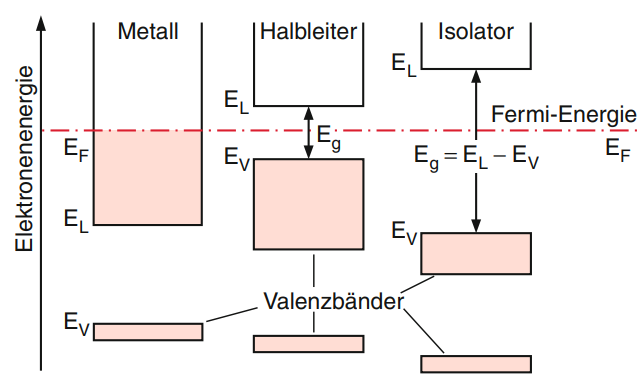
\includegraphics[width=0.7\textwidth]{figure/halbleiter.png}
    \caption{Übersicht des Bändermodells von Halbleitern. Dargestellt sind die Unterschiede zwischen Metallen, Halbleitern und Isolatoren \cite{demtroder}.}
    \label{fig:halbleiter}
\end{figure}

\subsection{Faraday-Effekt}
\label{ssec:faraday}